\section{Finite-Length Longitudinal PEEC}
\label{chapter:06}

% block-id: 06.peec_method.heading
\hypertarget{06.peec_method.heading}{}
\subsection{Finite-length longitudinal PEEC}

% block-id: 06.peec_method.p1
\hypertarget{06.peec_method.p1}{}
Longitudinal PEEC divides the cross-section into volume filaments, each carrying an axial complex current density uniform along its length. Ohmic resistance and finite-volume partial inductance follow \eqref{eq:E08}, forming Z=R+jωL before the common-port and total-current constraints in \eqref{eq:E04} are applied. The counts 1264 and 5024 denote volume-filament degrees of freedom in a continuous conductor. Differences between their currents represent internal current concentration within the longitudinal basis.

% block-id: 06.peec_method.p2
\hypertarget{06.peec_method.p2}{}
The longitudinal case has a nominal round-wire diameter of 2 mm. The m40 and m80 square filaments are 0.050 and 0.025 mm wide, giving actual cross-sectional areas of 3.16 and 3.14 mm². Sensitivity studies vary length, mutual integration, or self integration independently. The 1264-degree-of-freedom model uses one cross-section at lengths 0.16, 0.32, and 0.64 m. At fixed length, mutual quadrature order q is increased through 4, 6, and 8, while self-integration settings increase from 10/8 to 12/10. These pairs are AccuracyGoal and PrecisionGoal, the target absolute and relative precision digits. The 5024-degree-of-freedom model checks lengths 0.32 and 0.64 m and the same integration changes. Because the two cross-sectional discretizations have slightly different copper areas, each resistance is compared with its own equal-area Bessel reference; changes between discretizations include both discretization and area approximation.

% block-id: 06.peec_method.p3
\hypertarget{06.peec_method.p3}{}
The partial-inductance kernel includes magnetic coupling around finite conductors, whereas the Bessel solution gives the internal impedance of a long straight round wire. We compare their dissipative component Rac while retaining length and area conditions. The length study measures sensitivity of the current kernel and longitudinal basis. Transverse loops, curved strands, and actual end-current redistribution require extended degrees of freedom. The connection to FEM–PEEC coupling \cite{P03} lies in a joint field–circuit description; excitation, return, and field-feedback choices must be compared for each implementation.

% block-id: 06.peec_derivation.heading
\hypertarget{06.peec_derivation.heading}{}
\subsection{Longitudinal filament basis and kernel integration}

% block-id: 06.peec_derivation.p1
\hypertarget{06.peec_derivation.p1}{}
Within volume filament α, current density is constant at iα/Aα and directed axially. Volume integration of vector potential gives the induced electric field in a testing filament; integration along its length yields a symmetric partial-inductance matrix. Coincident points produce an integrable self-term singularity treated with dedicated precision settings, while mutual terms use a separate quadrature order. Ohmic resistance and jωL form the coupled matrix, solved jointly with common terminal voltage and total current. The basis determines the current directions represented by this model.

% block-id: 06.peec_results.heading
\hypertarget{06.peec_results.heading}{}
\subsection{Length and integration sensitivity of longitudinal PEEC}

% block-id: 06.peec_results.p1
\hypertarget{06.peec_results.p1}{}
For the 1264-degree-of-freedom model, resistances at 0.16, 0.32, and 0.64 m are 19.8992, 19.9586, and 19.9885 mΩ per axial metre. Consecutive length changes are 0.298640\% and 0.149482\%. The 5024-degree-of-freedom model changes by 0.148730\% from 0.32 to 0.64 m, as shown in Fig.~\ref{fig:peec_length}. Resistance changes decrease with increasing length, and all tested increments are below 1\%. The sequence characterizes sensitivity over the 0.16–0.64 m interval.

% block-id: 06.peec_results.p2
\hypertarget{06.peec_results.p2}{}
At 5024 degrees of freedom, Lz=0.64 m, mutual order q=4, and self-integration settings 12/10, Rac=\metric{peec_rac} mΩ per axial metre, Rac/Rdc=3.64472, and loss is 8.00510 W per axial metre. Resistance differs by 0.044582\% from the equal-area Bessel reference for this discretization. Fig.~\ref{fig:peec_cross_section} reconstructs the cross-sectional current distribution from saved filament currents and square cells, showing surface concentration within the conductor. These degrees of freedom discretize a continuous conductor; their current variation has a different meaning from current sharing among insulated strands.

% block-id: 06.peec_results.p3
\hypertarget{06.peec_results.p3}{}
Results for mutual order q=4\(\to\)6\(\to\)8 and self settings 10/8\(\to\)12/10 appear in Fig.~\ref{fig:peec_sensitivity}. Across both model sizes, the largest relative resistance change from mutual integration is 1.21×10⁻⁵ and the largest relative complex-current change is 1.60×10⁻⁵. Corresponding maxima for self integration are 6.75×10⁻¹¹ and 7.10×10⁻¹¹. Coarse-to-fine cross-sectional resistance changes at 0.32 and 0.64 m are 0.122127\% and 0.121376\%, respectively, and include changes in actual area. Thus integration settings have a smaller effect than length and cross-sectional discretization in these tests. Analytical references and sensitivities jointly support resistance calculation within the longitudinal model; actual end regions and transverse-current errors remain model-level research questions.

% block-id: 06.equation.E08
\hypertarget{06.equation.E08}{}
\hypertarget{E08}{}
\begin{equation}
\begin{gathered}
R_{\alpha\beta}=\delta_{\alpha\beta}\frac{L_z}{\sigma A_\alpha} \\
L_{\alpha\beta}=\frac{\mu}{4\pi A_\alpha A_\beta}\int_{V_\alpha}\int_{V_\beta}\frac{\hat{\mathbf t}_\alpha\cdot\hat{\mathbf t}_\beta}{|\mathbf r-\mathbf r'|}\,\mathrm dV\,\mathrm dV'
\end{gathered}
\tag{7}\label{eq:E08}
\end{equation}

% block-id: 06.figure.peec_cross_section
\hypertarget{06.figure.peec_cross_section}{}
\begin{figure}[!htbp]
\centering
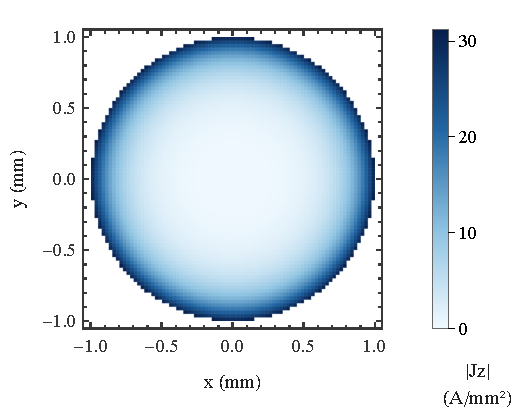
\includegraphics[width=\linewidth,height=.72\textheight,keepaspectratio]{../../assets/en/peec_cross_section.pdf}
\caption{Longitudinal PEEC cross-sectional current. Complex currents in square volume filaments reconstruct the RMS magnitude. The representative model contains 5024 longitudinal volume filaments and has axial length 0.64 m. Coordinates and material areas follow that level’s actual square-cell discretization.}
\label{fig:peec_cross_section}
\end{figure}

% block-id: 06.figure.peec_length
\hypertarget{06.figure.peec_length}{}
\begin{figure}[!htbp]
\centering
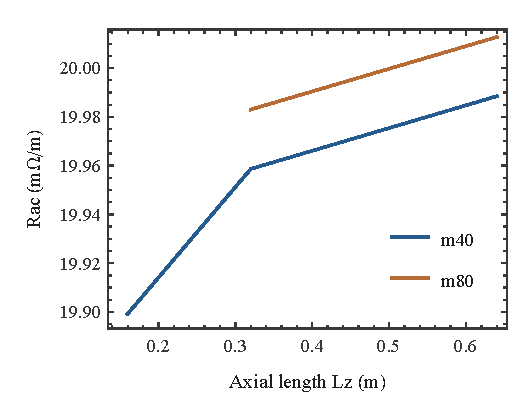
\includegraphics[width=\linewidth,height=.72\textheight,keepaspectratio]{../../assets/en/peec_length.pdf}
\caption{Longitudinal PEEC length sensitivity. Resistance per axial length is compared at archived lengths for the same cross-section. The 1264-degree-of-freedom model uses 0.16, 0.32, and 0.64 m, while 5024 degrees of freedom recheck the final two levels. Integration settings remain fixed within each length sequence.}
\label{fig:peec_length}
\end{figure}

% block-id: 06.figure.peec_sensitivity
\hypertarget{06.figure.peec_sensitivity}{}
\begin{figure}[!htbp]
\centering
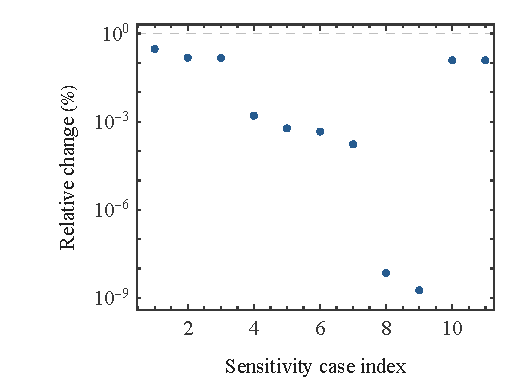
\includegraphics[width=\linewidth,height=.72\textheight,keepaspectratio]{../../assets/en/peec_sensitivity.pdf}
\caption{Longitudinal PEEC integration sensitivity. Mutual order and self accuracy are compared in separate single-factor tests. Mutual settings are q4, q6, and q8; self settings are 10/8 and 12/10. Comparisons retain the same cross-section and axial length.}
\label{fig:peec_sensitivity}
\end{figure}
